\documentclass[12pt]{article}

% Packages
\usepackage[margin=1in]{geometry}
\usepackage{fancyhdr}
\usepackage{amsmath, amsthm, amssymb, physics}
\usepackage{graphicx}

% Page Style
\fancypagestyle{plain}{
    \fancyhf{}
    \renewcommand{\headrulewidth}{0pt}
    \renewcommand{\footrulewidth}{0pt}
    \fancyfoot[R]{\thepage}
}
\pagestyle{plain}

% Problem Box
\setlength{\fboxsep}{4pt}
\newsavebox{\savefullbox}
\newenvironment{fullbox}{\begin{lrbox}{\savefullbox}\begin{minipage}{\dimexpr\textwidth-2\fboxsep\relax}}{\end{minipage}\end{lrbox}\begin{center}\framebox[\textwidth]{\usebox{\savefullbox}}\end{center}}
\newenvironment{pbox}[1][]{\begin{fullbox}\ifx#1\empty\else\paragraph{#1}\fi}{\end{fullbox}}

% Options
\renewcommand{\thesubsection}{\thesection(\alph{subsection})}
\allowdisplaybreaks
\addtolength{\jot}{4pt}
\theoremstyle{definition}

% Default Commands
\newtheorem{proposition}{Proposition}
\newtheorem{lemma}{Lemma}
\newcommand{\ds}{\displaystyle}
\newcommand{\isp}[1]{\quad\text{#1}\quad}
\newcommand{\N}{\mathbb{N}}
\newcommand{\Z}{\mathbb{Z}}
\newcommand{\Q}{\mathbb{Q}}
\newcommand{\R}{\mathbb{R}}
\newcommand{\C}{\mathbb{C}}
\newcommand{\eps}{\varepsilon}
\renewcommand{\phi}{\varphi}
\renewcommand{\emptyset}{\varnothing}
\newcommand{\pfrac}[2]{\left(\frac{#1}{#2}\right)}

% Extra Commands
\newcommand{\tsum}{\textstyle\sum\limits}

% Document Info
\fancypagestyle{title}{
    \renewcommand{\headrulewidth}{0.4pt}
    \setlength{\headheight}{15pt}
    \fancyhead[R]{Harry Coleman}
    \fancyhead[L]{GEOG 191 Lab 5}
    \fancyhead[C]{February 19, 2021}
}

% Begin Document
\begin{document}
\thispagestyle{title}



\begin{pbox}[1]
    Formulate the example shortest path problem reflected in the provided Xpress code (Network \#1).
\end{pbox}

For each pair of nodes $i, j$, we define $c_{ij}$ to be the cost of the directed edge $i \to j$. If there is no such edge, we define $c_{ij} = M$, where $M$ is a prohibitively high cost. This gives us the cost adjacency matrix
\[
    c = \mqty[
        M & 35 & 30 & M & M & M & M \\
        M & M & 12 & 18 & M & M & 39 \\
        M & M & M & M & 15 & M & M \\
        M & M & M & M & 5 & M & 16 \\
        M & M & M & M & M & 9 & M \\
        M & M & M & M & M & M & 18 \\
        M & M & M & M & M & M & M
    ].
\]
For each pair of nodes $i, j$, we define a binary decision variable $x_{ij}$, representing the choice of whether or not to include the edge from $i$ to $j$. Our objective function is the total cost of the selected path, i.e.,
\[
    Z = \tsum_{i=1}^{7} \tsum_{j=1}^{7} c_{ij}x_{ij}.
\]
To ensure that the path begins at node $1$, we use the constraint
\[
    \tsum_{j=1}^{7} x_{1j} = 1.
\]
This requires not only that some edge from node $1$ is selected, but exactly one such edge is selected, as each decision variable is binary. Similarly, we ensure that the path ends at node $7$ with the constraint
\[
    \tsum_{i=1}^{7} x_{i7} = 1.
\]
For each node which is not the start or end of the path, we must ensure that the number of edges directed into the node edge equals the number of edges directed out of the node. We implement this with the constraints
\[
    \tsum_{i=1}^{7} x_{ij} - \tsum_{i=1}^{7} x_{ji} = 0, \quad j = 2,\dots, 6.
\]
Together with the fact that exactly one edge starts at node $1$ and exactly one edge ends at node $7$, we know that a feasible solution to this problem will be a path. In conclusion, we obtain the following linear program
\[\begin{array}{lll}
    \textbf{Minimize} & Z = \tsum_{i=1}^{7} \tsum_{j=1}^{7} c_{ij}x_{ij} \\
    \textbf{Subject to} & \tsum_{j=1}^{7} x_{1j} = 1, \\
        & \tsum_{i=1}^{7} x_{i7} = 1, \\
        & \tsum_{i=1}^{7} x_{ij} - \tsum_{i=1}^{7} x_{ji} = 0, \quad &j = 2,\dots, 6, \\
        & x_{ij} \in \{0, 1\}, \quad &i, j = 1, \dots, 7.
\end{array}\]



\begin{pbox}[2]
    Depict the Xpress solution using network \#1 for this problem.
\end{pbox}

\begin{center}
    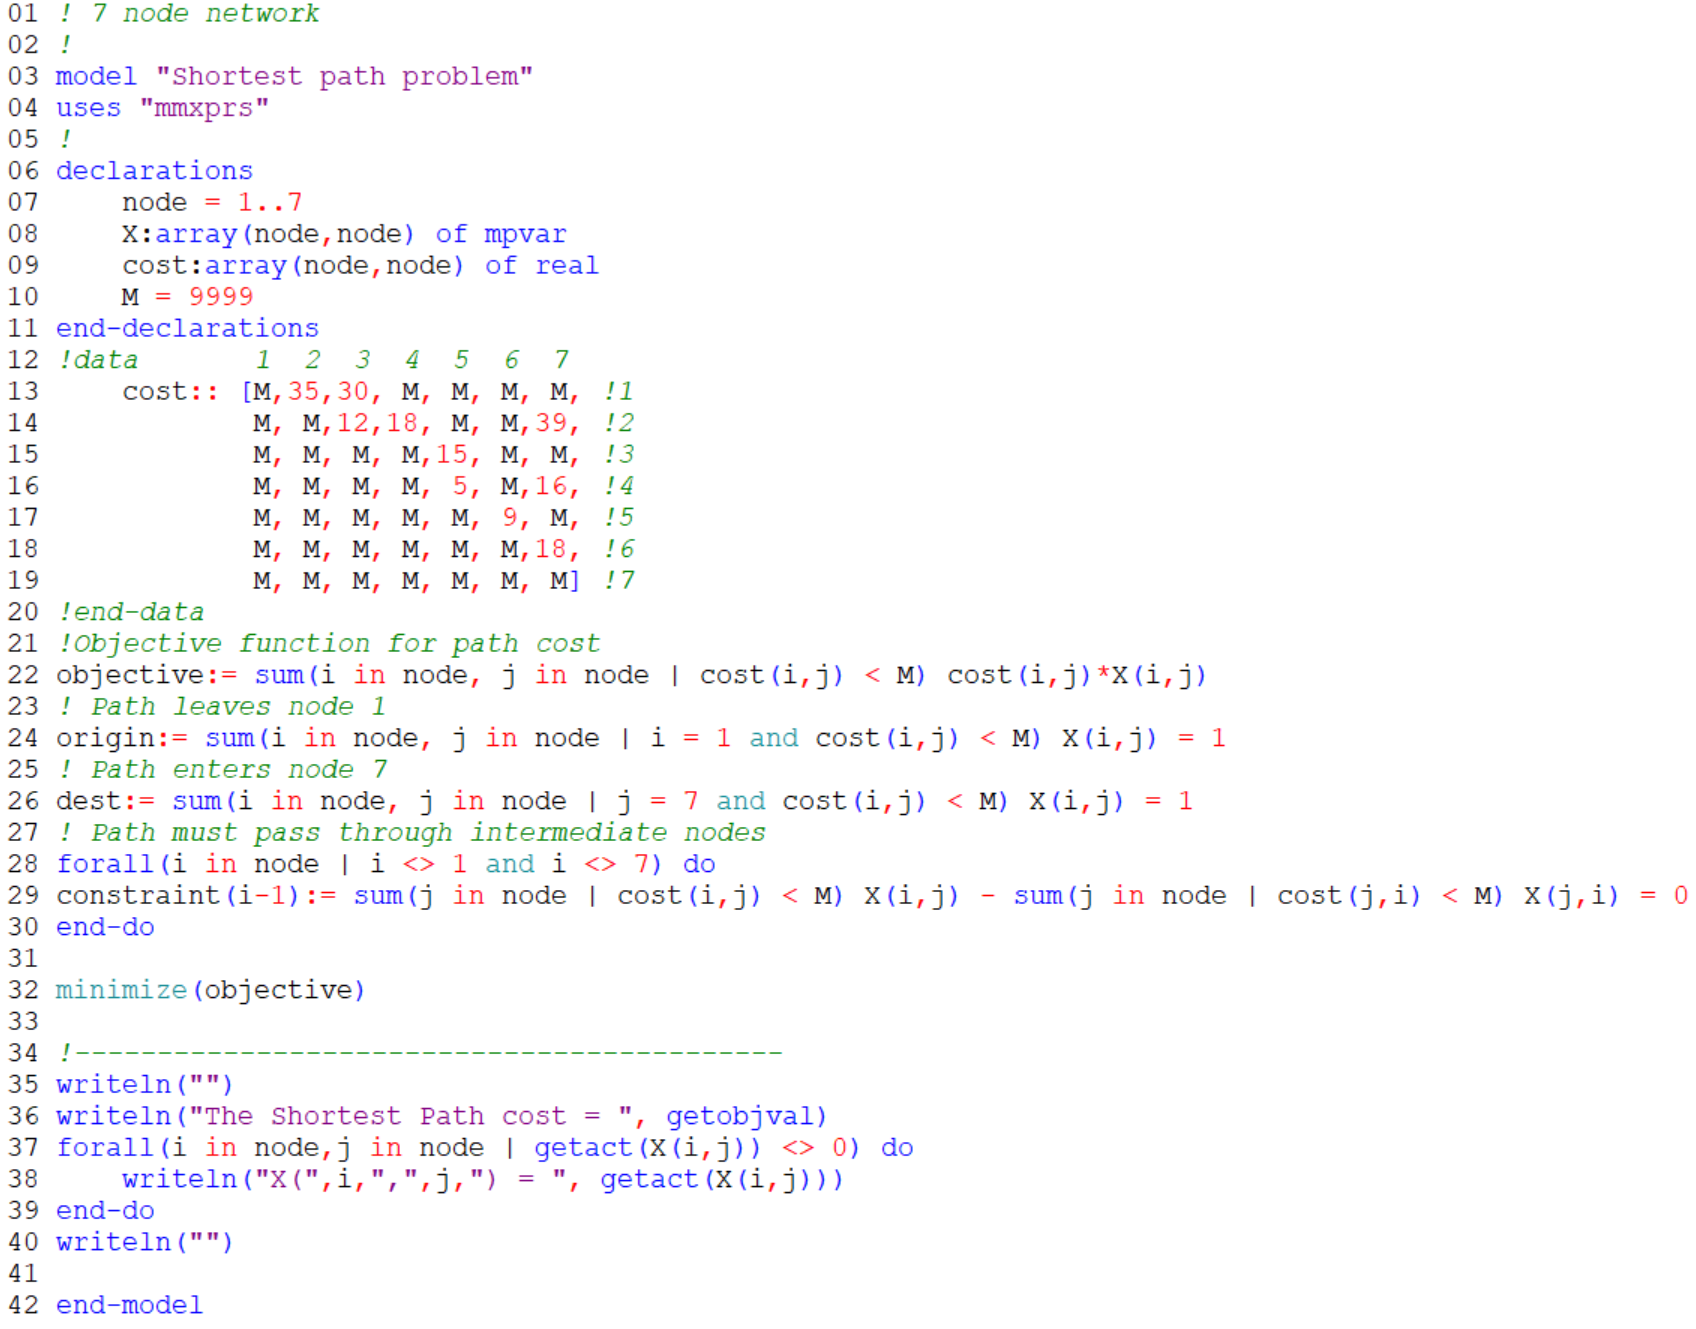
\includegraphics[width=\textwidth]{code1.png}
\end{center}
\begin{verbatim}
The Shortest Path cost = 69
X(1,2) = 1
X(2,4) = 1
X(4,7) = 1
\end{verbatim}
\begin{center}
    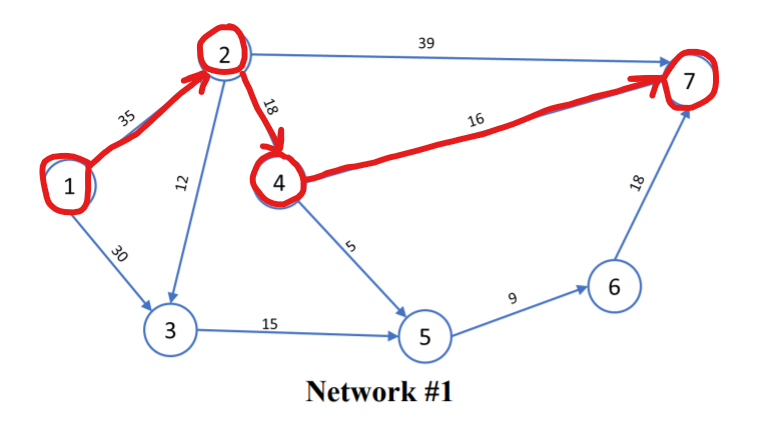
\includegraphics[width=0.6\textwidth]{sol1.png}
\end{center}




\begin{pbox}[3]
    What is the impact of a change to travel cost in Network \#1 between nodes 1 and 2, up to 45 units?
\end{pbox}

\begin{center}
    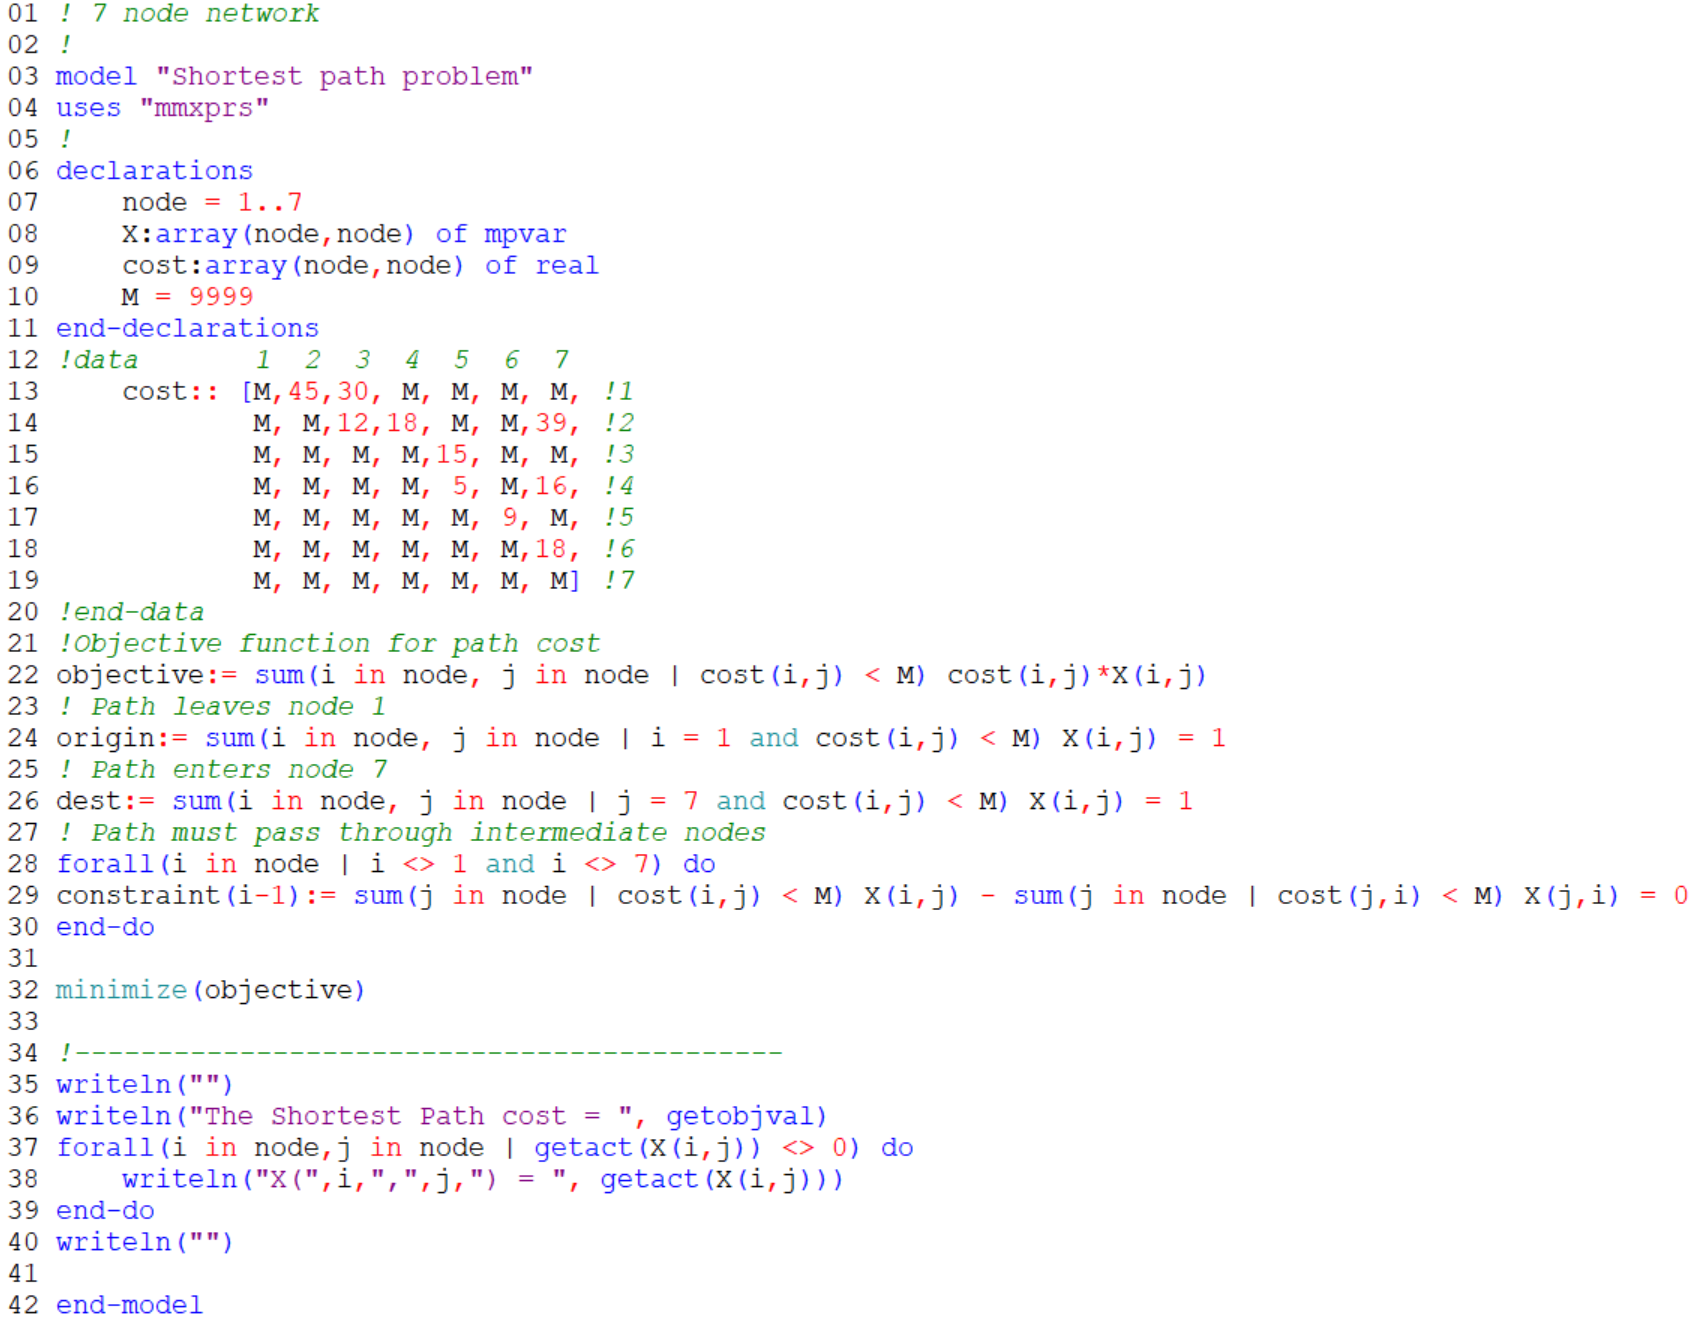
\includegraphics[width=\textwidth]{code2.png}
\end{center}
\begin{verbatim}
The Shortest Path cost = 72
X(1,3) = 1
X(3,5) = 1
X(5,6) = 1
X(6,7) = 1
\end{verbatim}
\begin{center}
    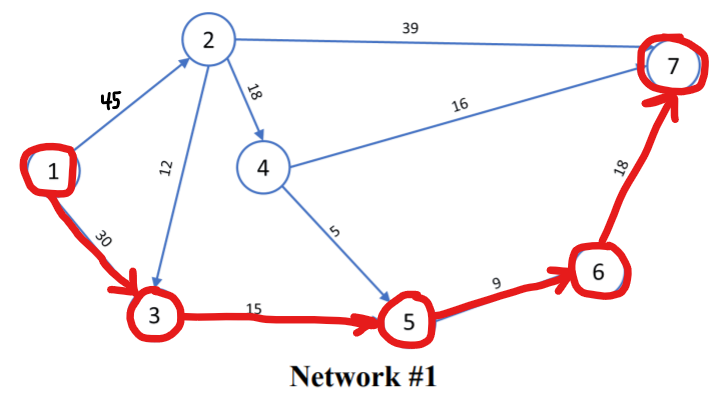
\includegraphics[width=0.6\textwidth]{sol2.png}
\end{center}


\begin{pbox}[4]
    If you modify the Xpress code to begin at node 6 and end at node 2 in Network \#1, what happens? Explain the reasons for this finding?
\end{pbox}

\begin{center}
    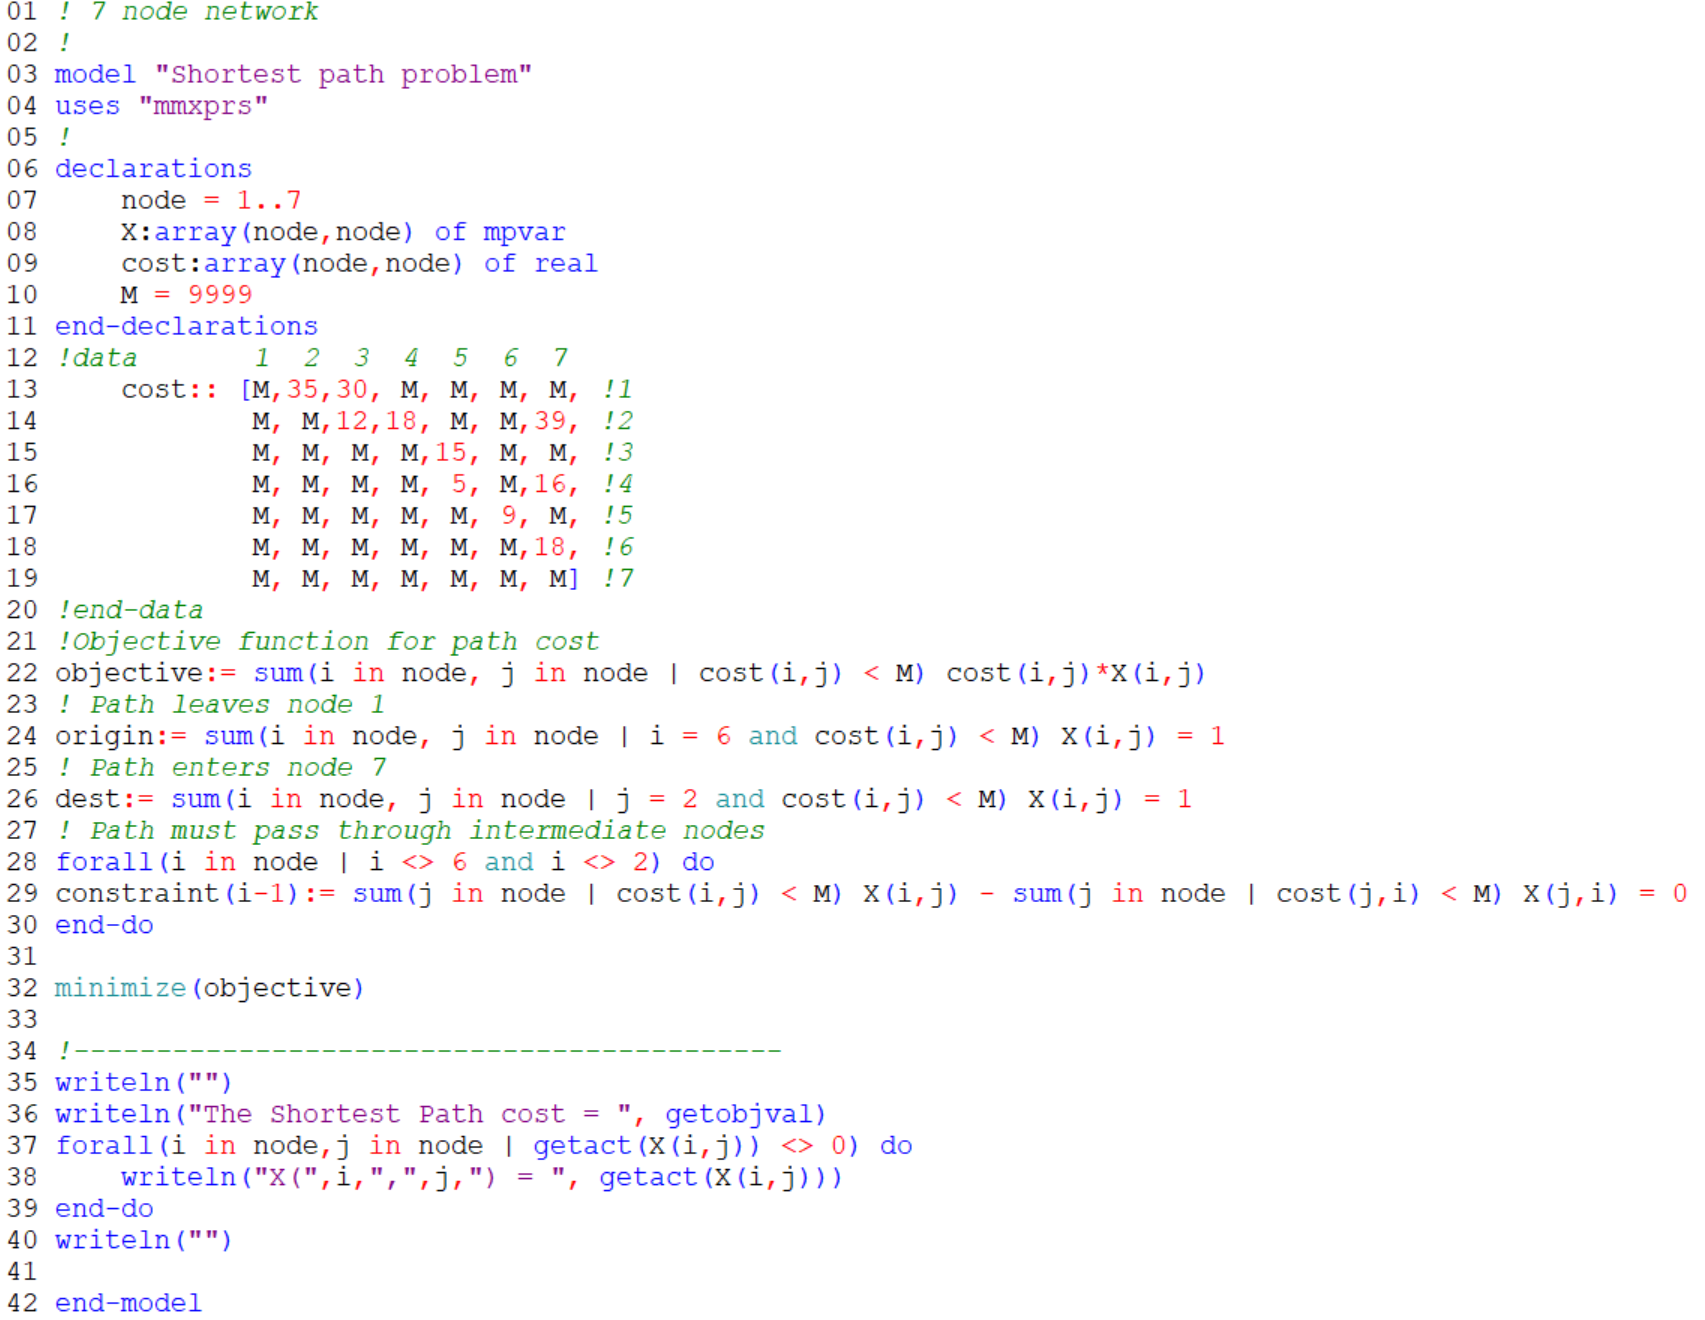
\includegraphics[width=\textwidth]{code3.png}
\end{center}

\begin{verbatim}
The Shortest Path cost = 0
\end{verbatim}

The only possible edge the path can start with is $6 \to 7$. But $7$ has no edges directed out of it, so the path terminates. That is, the problem is infeasible, which is what Xpress indicates when running the above code.



\newpage
\begin{pbox}[5]
    Structure and solve the shortest path problem for Network \#2, beginning at node 2 and ending at node 8.
\end{pbox}

We formulate this problem in the same way as network \#1, interpreting each edge as a pair of edges with opposite directions. Then we obtain the symmetric cost adjacency matrix
\[
    c = \mqty[
        M & 2 & 2 & M & 7 & M & 5 & M \\
        2 & M & 5 & 4 & M & M & M & M \\
        2 & 5 & M & 1 & 4 & 3 & M & M \\
        M & 4 & 1 & M & M & 4 & M & M \\
        7 & M & 4 & M & M & 1 & 6 & 5 \\
        M & M & 3 & 4 & 1 & M & M & 7 \\
        5 & M & M & M & 6 & M & M & M \\
        M & M & M & M & 5 & 7 & M & M
    ].
\]
Using the same variables and constraints as in Network \#1, but this time with $8$ nodes, we have the linear program
\[\begin{array}{lll}
    \textbf{Minimize} & Z = \tsum_{i=1}^{8} \tsum_{j=1}^{8} c_{ij}x_{ij} \\
    \textbf{Subject to} & \tsum_{j=1}^{8} x_{2j} = 1, \\
        & \tsum_{i=1}^{8} x_{i8} = 1, \\
        & \tsum_{i=1}^{7} x_{ij} - \tsum_{i=1}^{7} x_{ji} = 0, \quad &j = 1, 3, \dots, 7, \\
        & x_{ij} \in \{0, 1\}, \quad &i, j = 1, \dots, 8.
\end{array}\]
We implement this problem in Xpress, as before.

\begin{center}
    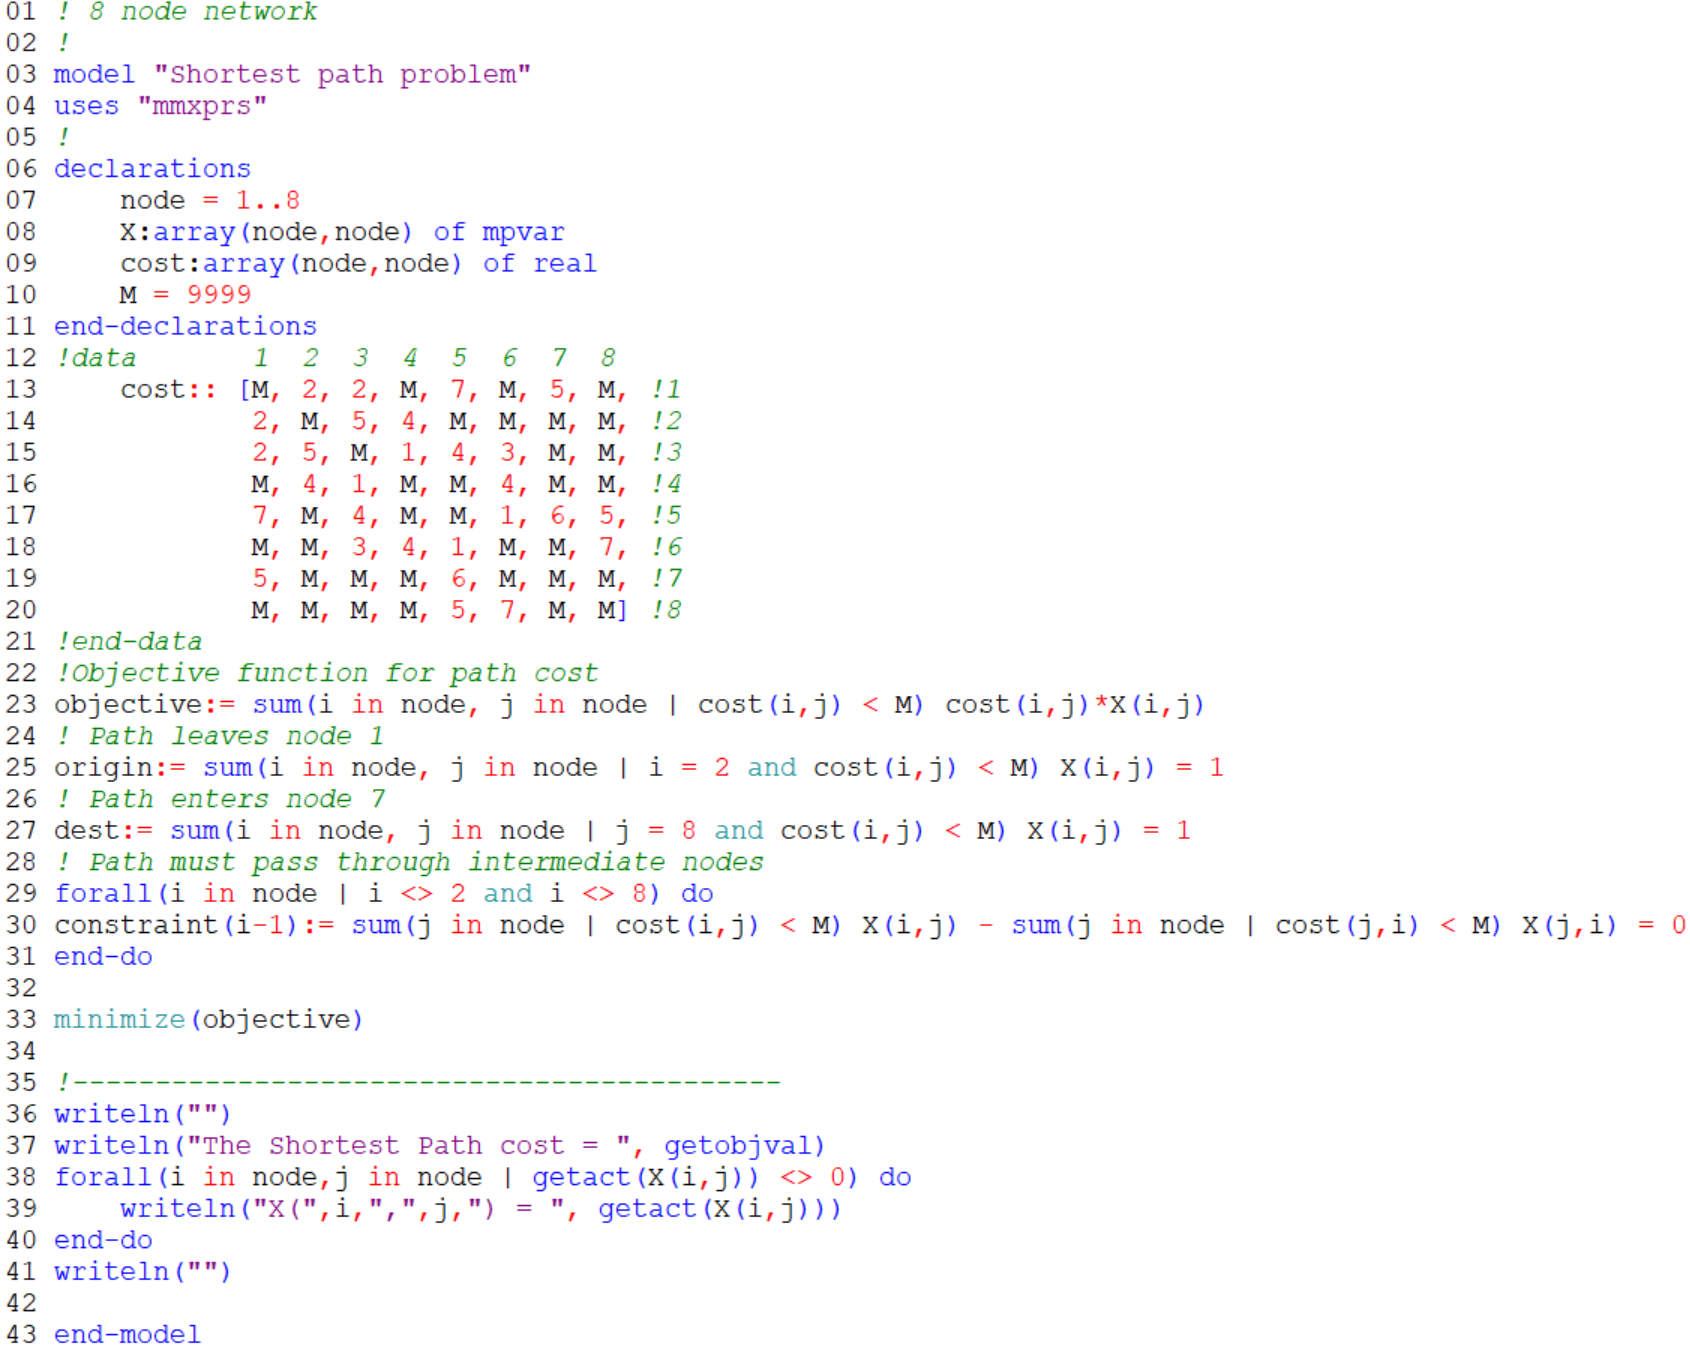
\includegraphics[width=\textwidth]{code4.png}
\end{center}

\begin{verbatim}
The Shortest Path cost = 13
X(1,3) = 1
X(2,1) = 1
X(3,5) = 1
X(5,8) = 1
\end{verbatim}

\begin{center}
    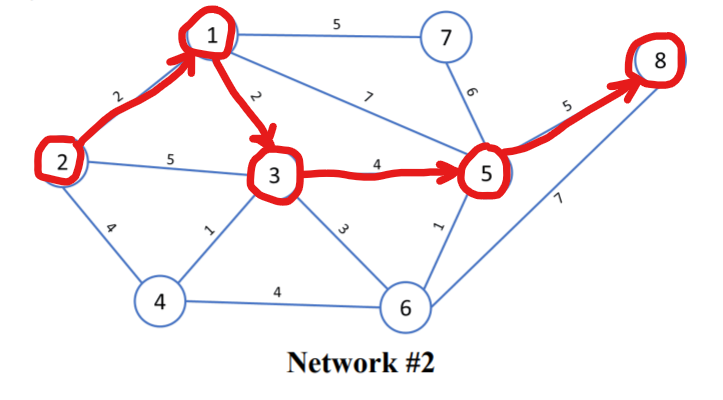
\includegraphics[width=0.6\textwidth]{sol4.png}
\end{center}



\newpage
\begin{pbox}
    For an area that you are familiar with, create a network with arc travel costs over which you
    would structure a corresponding shortest path problem to help you make a good routing decision.
    You may want to use Google Maps to help you with this.
    \begin{itemize}
        \item Pick one source and one destination, within a mile
        \item Digitize relevant segments between the two points; be cognizant of one-ways
        \item Assign travel costs on segments
        \item Represent the intersections, source and destination as nodes and paths as edges within a network
    \end{itemize}
\end{pbox}

In the following network, we want a path from node $1$ to node $9$. The cost for each edge is its length in feet, shown on the map.

\begin{center}
    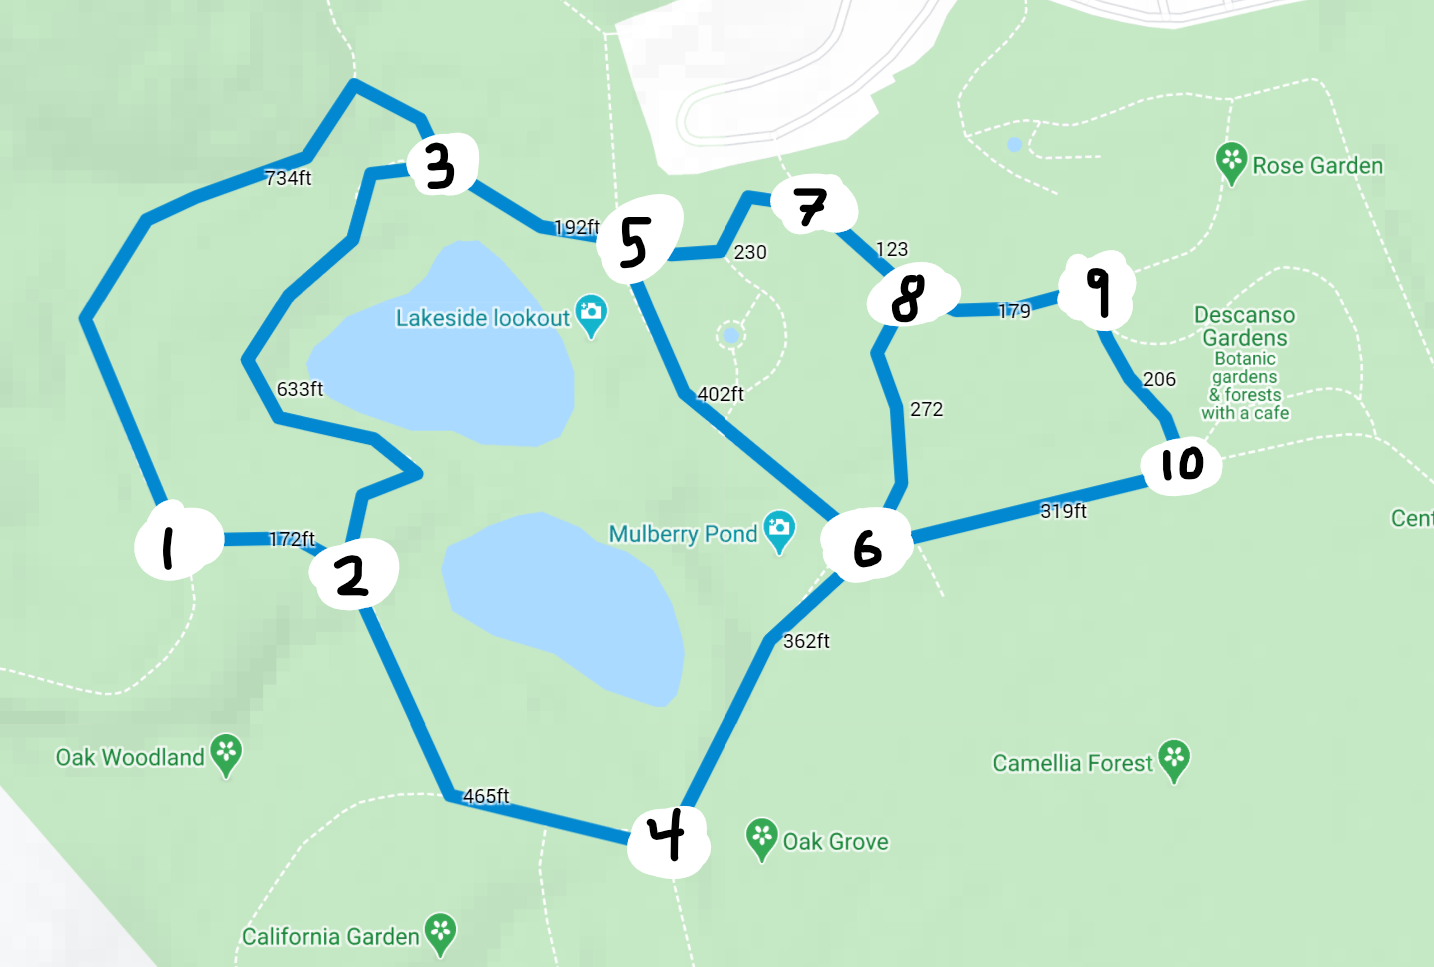
\includegraphics[width=\textwidth]{googlemap.png}
\end{center}


\newpage
\begin{pbox}[8]
    For the network you created, what is the shortest route you would recommend from the origin to destination? How does this compare to what is identified by Google Maps?
\end{pbox}

Without looking at any numbers, my initial guess for the shortest path is $(1, 2, 4, 6, 8, 9)$. However, Google recommends the path $(1, 3, 5, 7, 8, 9)$, as seen below.

\begin{center}
    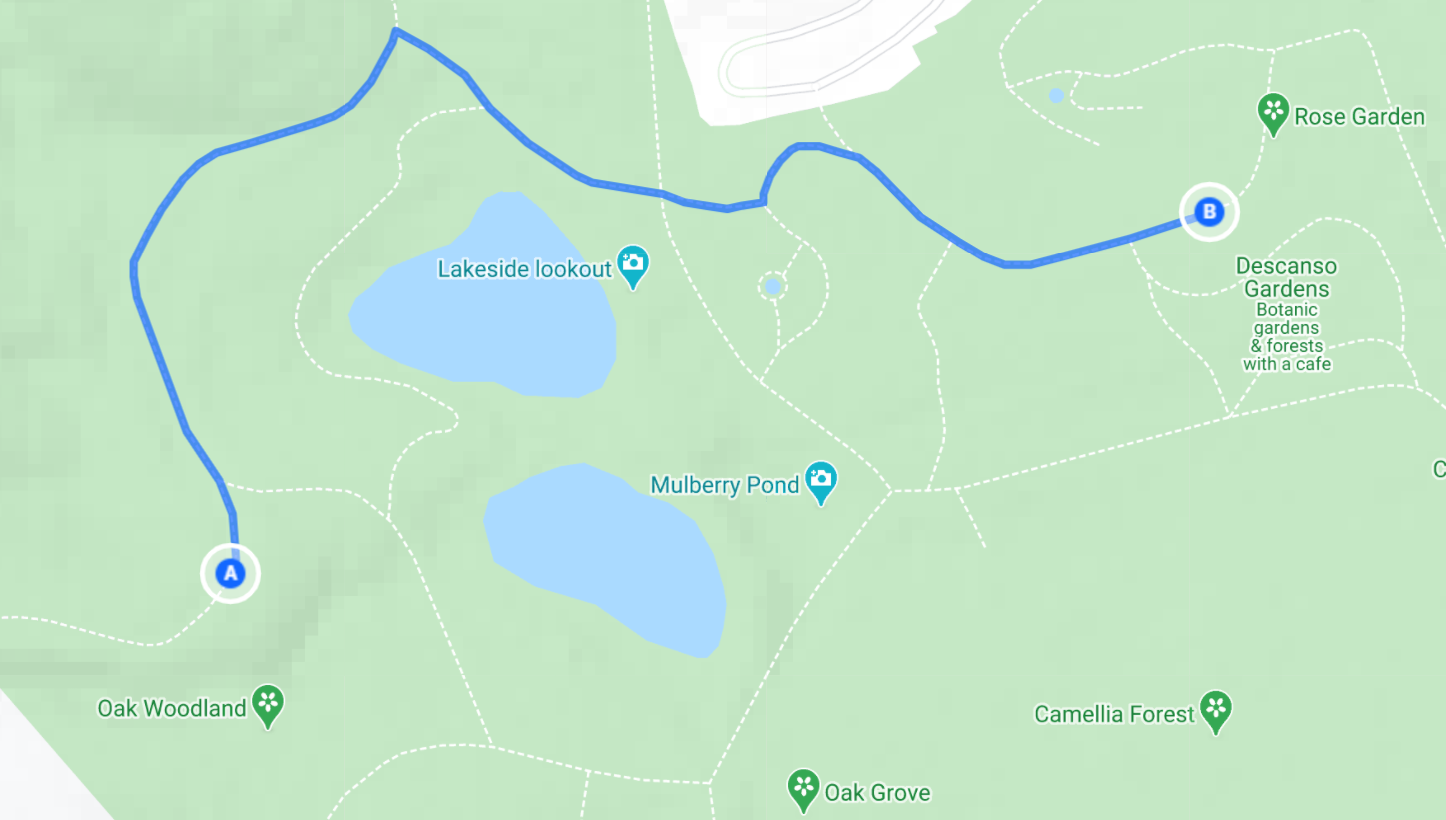
\includegraphics[width=\textwidth]{googlesol.png}
\end{center}

Implementing the problem in Xpress, we obtain the following results.

\begin{center}
    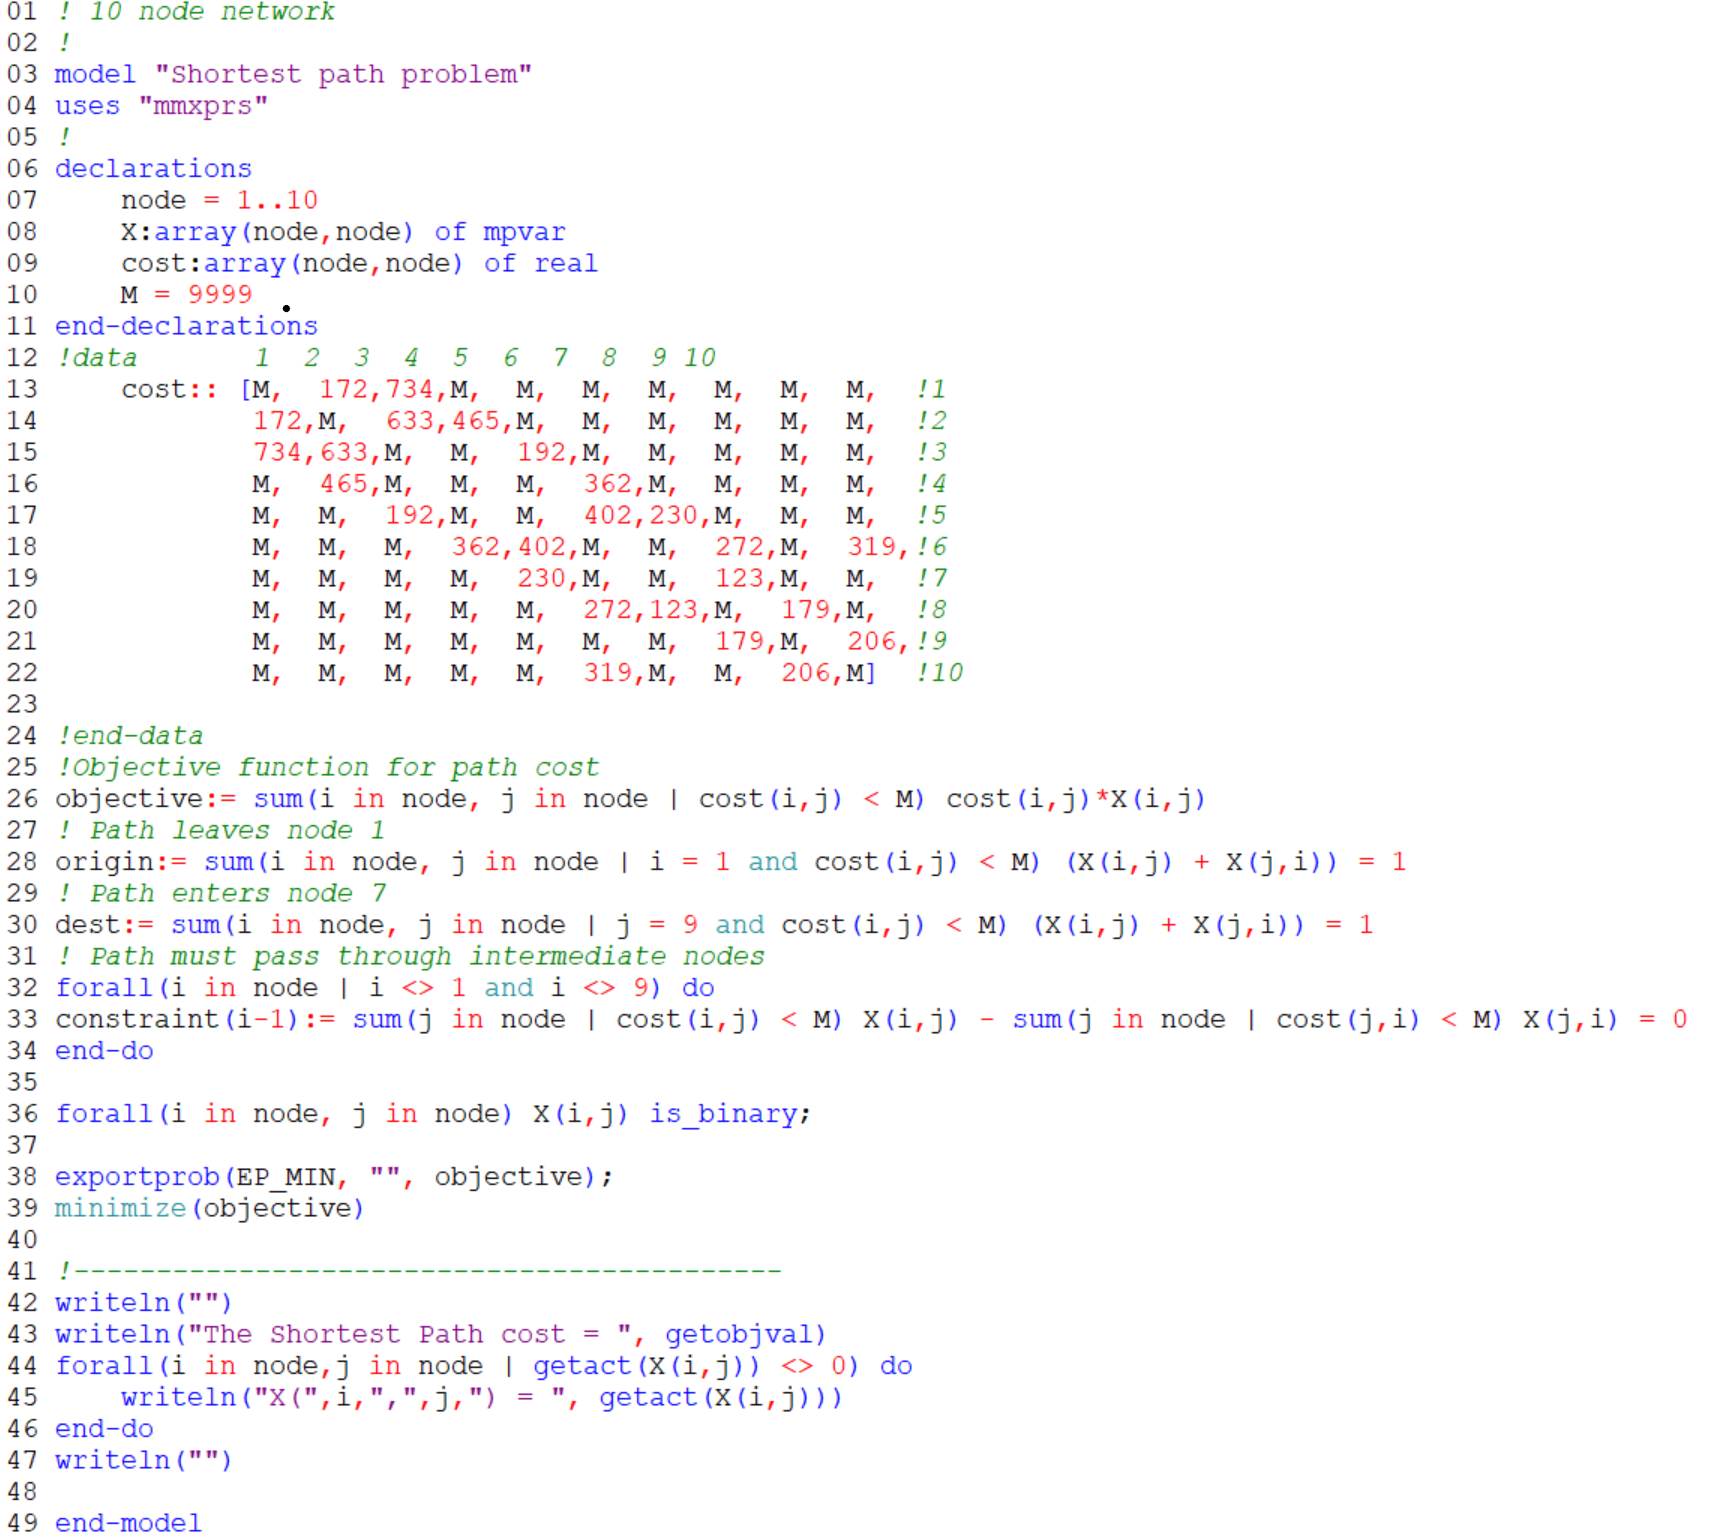
\includegraphics[width=0.9\textwidth]{codeg.png}
\end{center}

\begin{verbatim}
The Shortest Path cost = 1450
X(2,1) = 1
X(4,2) = 1
X(6,4) = 1
X(8,6) = 1
X(9,8) = 1
\end{verbatim}

\begin{center}
    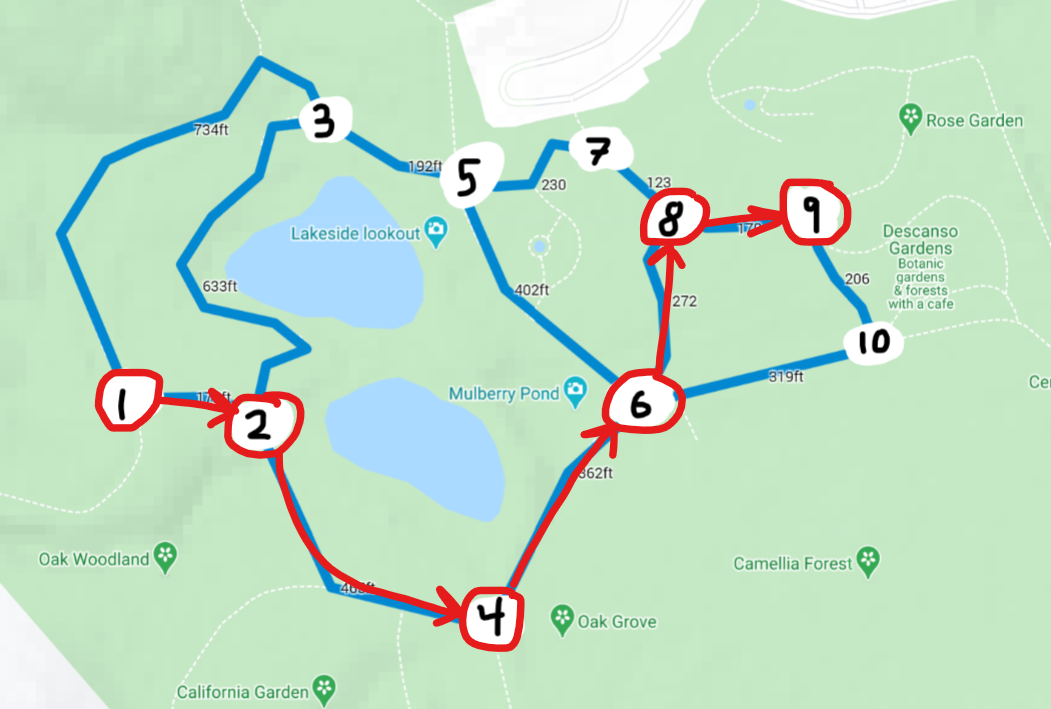
\includegraphics[width=0.5\textwidth]{solg.png}
\end{center}

\end{document}